\chapter{The Hypercompressor}
\label{ch:hypercompressor}

The motivation for Hypercompression came during the development of
Vocal Vibrations, an interactive music installation about the human
voice and about engaging the public in singing.\cite{Holbrow2014} The
project featured a Music Concr\`{e}te composition, \textit{The Chapel}
by Tod Machover, which was mixed in a 10 channel surround sound
format and played throughout the installation. During the mixing
process, I noticed an important surround sound tool missing from my
mixing workflow. When mixing in mono or stereo, audio
compression\marginnote{Unless noted otherwise, ``compression'' is used
  in this thesis to describe dynamic range compression, as opposed to
  data compression.} lets us meticulously shape and balance sounds in
time. I found myself wishing I could shape and position sounds in
space just as easily.

\section{Building on the Compression Paradigm}
The design, implementation, and use of traditional dynamic range
compression is well documented in the
literature,\cite[]{Giannoulis2012,Case2007,Deruty2014} so we will
describe dynamic range compression only as much as is needed to
explain the foundation for \thesis. Imagine we are mixing a vocal pop
performance, and during the verse our vocalist is singing moderately
loud, or \textit{mezzo-forte}. At the beginning of the chorus, our
singer wants a full and powerful sound, so she adjusts the dynamic to
very loud, or \textit{fortissimo}. However, the new louder dynamic
interrupts the balance between the vocals and the other instruments in
our mix. We like the powerful sound of our singer's
\textit{fortissimo} performance, but our balance would be improved if
we had the volume of a \textit{forte} performance instead. One option
is to manually turn down the vocalist during the chorus, which in some
cases this is the best solution. When we want more precise control, we
can use a compressor.

\subsection{Traditional Compression}
\label{sec:trad-compr}
A compressor is essentially an automated dynamic volume control.  Most
compressors include at least four basic parameters in the user
interface that allow us to customize its behavior: \textit{threshold},
\textit{ratio}, \textit{attack time}, and \textit{release time}.  We
can send our vocalist's audio signal through a compressor, and
whenever her voice exceeds the gain level set by our threshold
parameter, the signal is automatically attenuated. As the input signal
further exceeds the threshold level, the output is further attenuated
relative to the input signal. The ratio parameter determines the
relationship between the input level and output level as shown in
figure~\ref{fig:comp-ratio}.

\begin{marginfigure}
  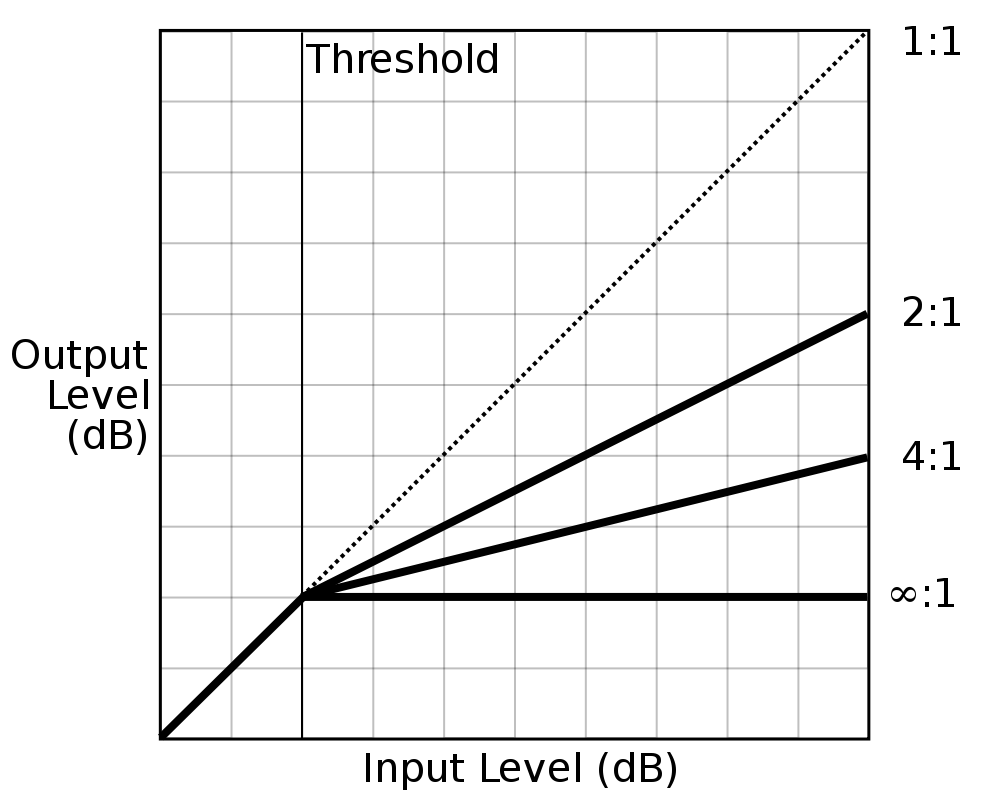
\includegraphics[]{CompressionRatio.png}
  \caption{``Compression ratio'' by Iain Fergusson. Licensed under
     Public Domain via Wikimedia Commons 
     \url{https://commons.wikimedia.org/wiki/File:Compression_ratio.svg\#/media/File:Compression_ratio.svg}
   }
  \label{fig:comp-ratio}
\end{marginfigure}

Threshold and ratio settings are essential for controlling dynamic
range, but the power and creative flexibility of the compressor comes
with the attack time and release time parameters. These parameters
determine the speed at which the compressor attenuates (attack time)
and disengages (release time) when the input signal exceeds the
threshold. By adjusting the attack and release times, we can change
the temporal focus of the compressor.
\begin{itemize}
\item Perhaps we want the compressor to engage or disengage at the
  time scale of a musical phrase. We could set our attack time long
  enough to let transients through without engaging the compressor
  significantly (try 20 milliseconds). If our release time is quite
  long (try 300 milliseconds), and we set our threshold and ratio
  carefully, we might be able to convince the compressor to smooth
  musical phrases.
\item If we want our compressor to focus on syllables instead of
  phrases, we can shorten our attack and release times (try 10
  milliseconds and 40 milliseconds respectively). When the compressor
  engages and disengages at each syllable, it imparts a different
  quality (sometimes described as ``punch'').
\item If we reduce our attack and release parameters enough, we can
  instruct our compressor to engage and disengage at the time scale of
  an audio waveform, compressing individual cycles. This will distort
  an audio signal, adding odd order harmonics,\sidenote{Not every
    compressor model can react quickly enough to distort a
    waveform. The Dbx 160 and Teletronix LA2A are known to be fast
    enough to distort.} and imparting an entirely different quality.
\end{itemize}
The attack and release times listed here are a rough guide only.  The
exact function of these parameters varies from one model of compressor
to another, and results also depend on the audio input material and
on the threshold and ratio settings. The results of audio
compression can sometimes be characterized better by a feeling than a
formula.

\begin{figure*}
  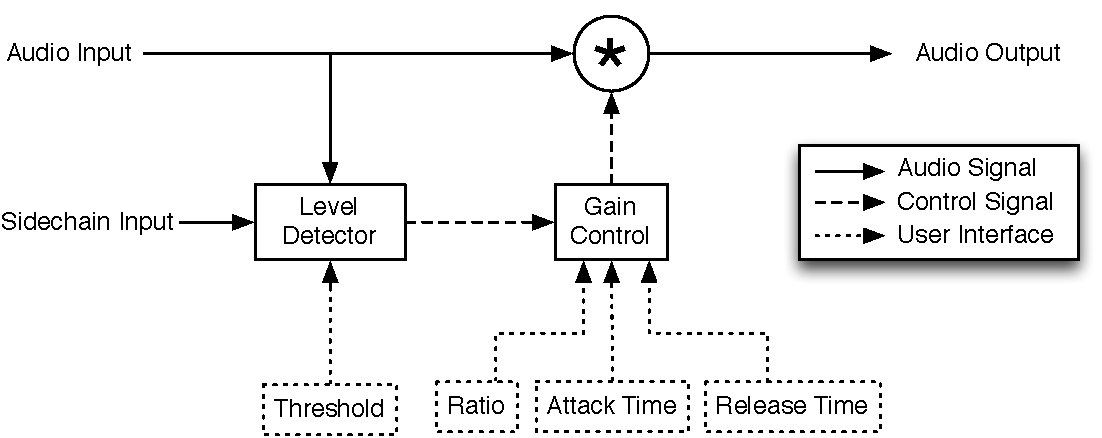
\includegraphics[width=\linewidth]{hypercomp/SimpleCompressor.pdf}
  \caption{Block diagram of a simple traditional dynamic range
    compressor.}
  \label{fig:comp-block}
\end{figure*}

\subsection{Side-Chain Compression}
\label{sec:side-chain-compr}
Compressors often have an additional operational mode that is the
primary inspiration for Hypercompression. We know that compressors
automatically reduce the gain of a signal that exceeds a given
threshold. Some compressors allow us to attenuate the level of a
signal when a \emph{different} signal exceeds the threshold
level. Models that suports side-chain compression have a second audio
input. When we switch the compressor into side-chain mode, the
compressor attenuates the first signal only when the second signal
exceeds the threshold.

Side-chain compression is often used to moderate the balance of kick
drum and bass guitar. If the bass guitar is briefly attenuated just
enough just the right amount each time the kick drum hits, we can set
the kick and bass guitar at exactly the gain levels we want without
one masking the other. Because the bass guitar is only briefly
attenuated, it will not be perceived as any quieter.

In this example we use the kick drum to create a gain envelope for our
bass guitar. The kick \emph{pushes} the bass to make room for
itself. The attack time and release time parameters give control over
this behavior in the temporal domain. The next step is to
expand this model to add control in the spatial domain.

\section{Ambisonics}
\label{sec:ambisonics}
Ambisonics is a technique for encoding and decoding three-dimensional
surround sound audio.\cite[-15mm]{Gerzon1973,Gerzon1985} Ambisonic
audio differs from other surround sound formats like $5.1$ and $7.1$
in that it does not depend on a particular speaker configuration. An
ambisonic recording can be decoded on any surround sound speaker
configuration without disarranging the spatial contents of the audio
recording.

Imagine we use an omnidirectional microphone to record an acoustic
instrument at a sample rate of 44.1 kHz. We sample and record 44100
samples every second that represent the air pressure at the microphone
capsule during the recording. Our omni-directional microphone is
designed to treat sound arriving from all angles equally. The
omnidirectional microphone sums together sounds arriving from all
angles and the acoustic directional information is lost.

If we want to encode, decode, transmit, or play audio that preserves
full sphere 360 degree information, ambisonics offers a solution.
Ambisonic audio uses \textit{spherical harmonics} to encode surround
sound audio that preserves the direction-of-arrival information that
discrete channel recordings (such as mono and stereo) cannot fully
capture.

\subsection{Spherical Harmonics}
\label{sec:spherical-harmonics}
We know that we can construct any monophonic audio waveform by summing
a (possibly infinite) number of harmonic sine waves (Fourier
series).\sidenote{An excellent description of the transformation between
  the time domain and frequency domain can be found at
  \url{http://betterexplained.com/articles/an-interactive-guide-to-the-fourier-transform/}}
For example, by summing odd \textit{order} sine harmonics at a given
frequency $f$, $(1f, 3f, 5f, 7f, \ldots )$, we generate a square wave
with fundamental frequency $f$. As the order increases, so does the
temporal resolution of our square wave.

By summing sinusoidal harmonics, we can generate any continuous
waveform defined in two dimensions (one input parameter and one
output). Similarly, by summing \emph{spherical harmonics}, we can
generate any continuous shape defined over the surface of a
three-dimensional sphere (two input parameters, or polar angles, one
output). Where a traditional monophonic audio encoding might save one
sample 44100 times per second, an ambisonic encoding would save one
sample \emph{for each spherical harmonic} 44100 times per second. This
way we capture a three-dimensional sound image at each audio sample.
The number of spherical harmonics we encode is determined by our
\textit{ambisonic order}. As our ambisonic order increases, so does
the angular resolution of our result on the surface of the sphere.

\subsection{Spherical Harmonic Definition}
For encoding and decoding ambisonics, the convention is to use the
real portion of spherical harmonics as defined in
equation~\ref{eq:spherical}, where:
\begin{itemize}
\item $Y_{n}^{m}(\varphi,\vartheta)$ is a spherical harmonic that
is:\marginnote{Some literature on spherical harmonics swaps the names
  of \textit{order} and \textit{degree}. In this thesis we use
  $Y_{order}^{degree}$. In literature where $Y_{degree}^{order}$ is
  used, the function of the subscript and superscript remain
  unchanged; only the names are inconsistent.}
\begin{itemize}
\item of order, $n$
\item of degree, $m$
\item defined over polar angles $(\varphi, \vartheta)$
\end{itemize}
\item $N_n^{|m|}$ is a normalization factor.\sidenote{In ambisonic
    literature (and software), there are multiple incompatible
    conventions for the normalization of spherical harmonics. The
    Hypercompressor uses the \textit{Furse-Malham} (FuMa)
    normalization convention.}
\item $P_n^{|m|}$ is the associated Legendre function of order $n$
  and degree $m$.
\end{itemize}
\begin{equation}
Y_{n}^{m}(\varphi,\vartheta)=N_n^{|m|}P_n^{|m|}(\sin{\vartheta})
\begin{cases}\label{eq:spherical}
\sin{|m|\varphi},&  \text{for $m<0$}\\  
\cos{|m|\varphi},& \text{for $m\geq 0$}\\
\end{cases}
\end{equation}
Given equation~\ref{eq:spherical}, we can define an ambisonic
audio recording as:
\begin{equation}
f(\varphi,\vartheta,t)=\sum\limits_{n=0}^N\sum\limits_{m=-n}^nY_n^m(\varphi,\vartheta)\phi_{nm}(t)
\label{eq:ambisonics}
\end{equation}
Where:
\begin{itemize}
\item $\varphi$ and $\vartheta$ describe the polar angle of sound
  arrival in two dimensions.\sidenote{Note that ambisonics uses polar
    angles to describe the angle of arrival of sound. These are
    similar to spherical coordinates, minus the inclusion of
    \textit{radial distance}. Distance is not part of the ambisonic
    specification.}
\item $t$ is time
\item $\phi_{nm}(t)$ are our \textit{expansion coefficients}, described
  below.
\end{itemize}
\begin{figure}[h]
  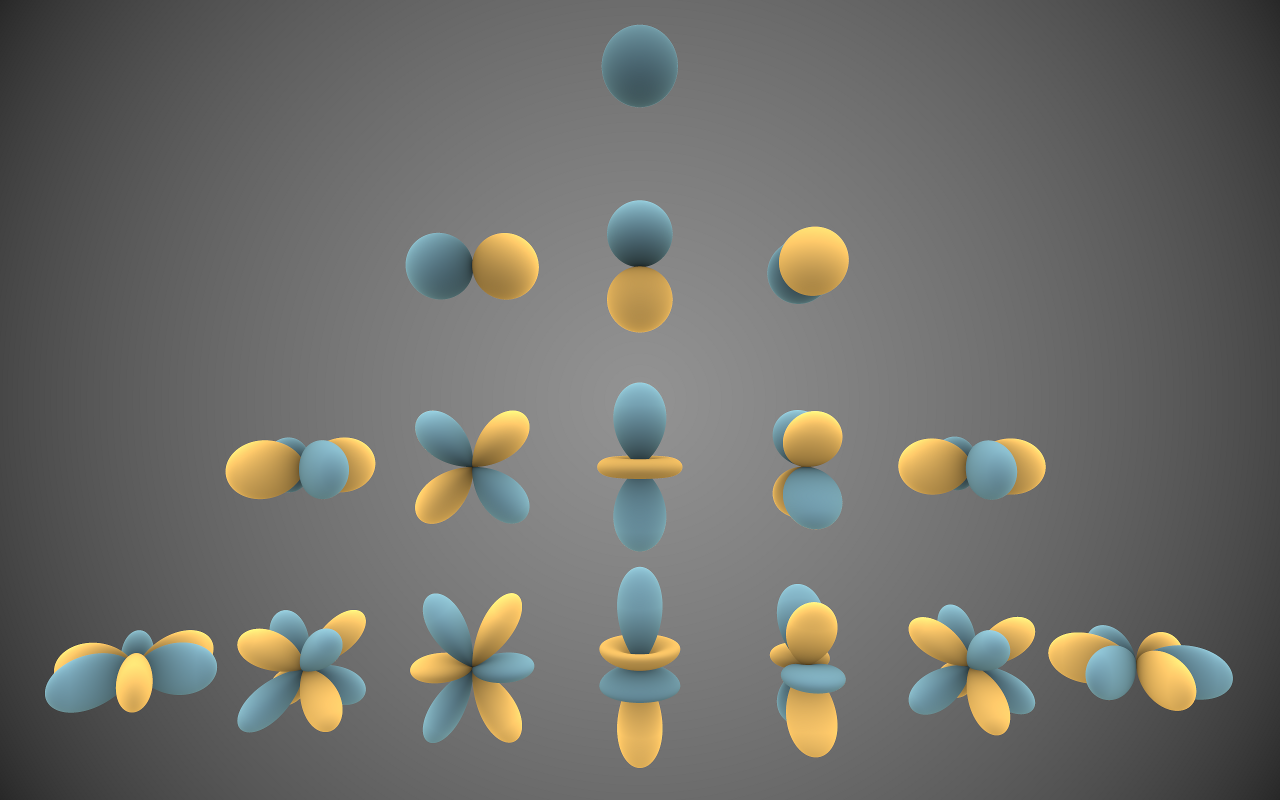
\includegraphics[width=\linewidth]{SphericalHarmonics.png}
  \caption{Spherical harmonics $0$th order (top row) through $3$rd
    order (bottom row). This for image shows the output of
    $Y_{n}^{m}(\varphi,\vartheta)$ for $n=0,n=1,n=2,$and $n=3$. The
    distance of the surface from the origin shows the value at that
    angle. Darker blue regions are positive, while lighter yellow
    regions are negative. Image credit: Ingo Quilez, licensed under
    \textit{Creative Commons Attribution-Share Alike 3.0 Unported}.}
  \label{fig:spherical-harmonics}
\end{figure}

\subsection{Spherical Harmonic Expansion Coefficients}
\label{sec:spher-harm-expans}
In our monophonic recording example, we save just one digital sample
44100 times per second, with each saved value representing the air
pressure at a point in time. We know that by summing the correct
combination of spherical harmonics, we can describe any continuous
function over the surface of a sphere. Instead of sampling air
pressure directly, we sample a coefficient describing the weighting of
each spherical harmonic 44100 times per second. The resulting sphere
encodes the pressure including the direction of arrival
information. The weighting coefficients or \textit{expansion
  coefficients} are recorded in our audio file instead of values
representing air pressure directly. Now, by summing together our
weighted spherical harmonics, we can reconstruct the fluctuations in
pressure including the angle of arrival information. We can recall
this snapshot of information at our 44.1 kHz audio sample rate.

\subsection{Ambisonic Encoding}
\label{sec:usage}
There are two ways to create an ambisonic recording. First, we can use
a soundfield microphone to record an acoustic soundfield. Soundfield
microphones like the one developed by Calrec Audio can capture angle
of arrival information with the spatial resolution of first order
ambisonics.\cite[-1in]{Ferrar1979} Alternatively, we can algorithmically
encode pre-recorded sources, creating virtual sources in an
ambisonic bus.\cite[-0.4in]{Malham1995}

\section{Ambisonic Conventions used for Hypercompression}
\label{sec:ambis-conv-used}
This thesis follows ambisonic convention for describing axis of
rotation. The x-axis points forward, the y-axis point left, and the
z-axis points up. Polar angles are used to describe orientation with
$0\degree$ azimuth being forward, and increasing as we move to the
right. $0\degree$ elevation also points forward, and increases as we
move upward, with $90\degree$ being strait up along the z-axis. When
working with ambisonics, multiple incompatible conventions exist for
ordering and normalizing spherical harmonics.\cite{Nachbar2011b} The
Hypercompressor uses \textit{Furse-Malham} normalization
(FuMa)\cite{Malham2003}, and first order ambisonics with
\textit{B-format}\cite{Hollerweger2008} channel ordering. B-format
ordering labels the four first-order ambisonic channels as W, X, Y,
and Z, with W being the spherical harmonic of order zero and degree zero,
and X, Y, and Z being the pressure gradient components along their
respective axes. 

\section{Hypercompressor Design}
\label{sec:hypercomp-design}
\begin{figure*}
  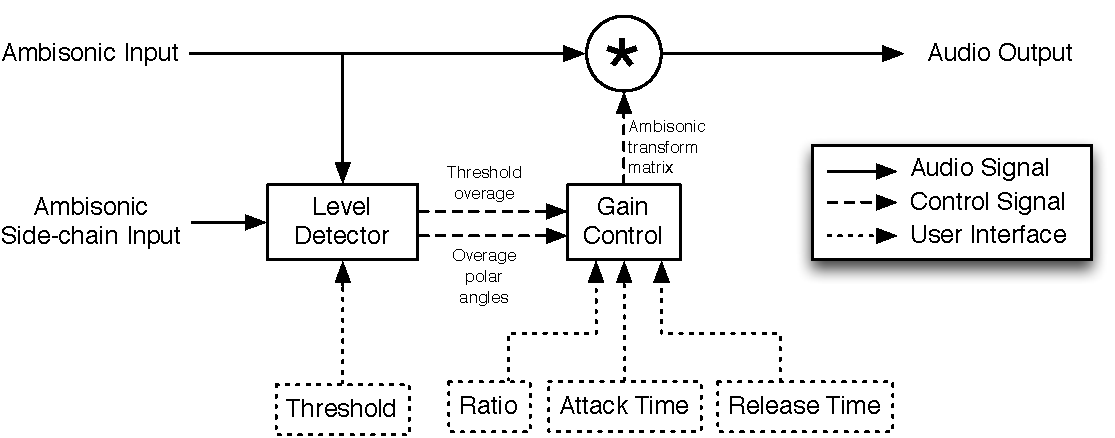
\includegraphics[width=\linewidth]{hypercomp/AmbisonicCompressor.pdf}
  \caption{Hypercompressor block diagram}
  \label{fig:hypercomp-block}
\end{figure*}
\noindent The Hypercompressor (or ambisonic compressor) combines the traditional
model of compression with the surround sound capability of
ambisonics. Given ambisonic input, and an optional ambisonic
side-chain input, the ambisonic compressor is intended to process our
input material in one of two modes:
\begin{enumerate}
\item Standard mode: We set a compression threshold, similar to on a
  traditional compressor. When a region in our surround sound input
  material exceeds the set threshold, the compressor engages and
  attenuates only that region.
\item Side-chain mode: This mode takes advantage of a second ambisonic
  input to our signal processor. When the gain of spatial region in
  our secondary input exceeds our threshold, we attenuate that same
  region in the the main input, and output the results.
\end{enumerate}
In both modes, our ambisonic compressor must attenuate and release
attenuation according to the attack time and release time
parameters. The block diagram for our new hypercompressor
(figure~\ref{fig:hypercomp-block}) can remain largely unchanged from
the the block diagram for our traditional compressor in
figure~\ref{fig:comp-block}. The most important changes are:
\begin{itemize}
\item Our audio signals must be updated to handle encoded
  ambisonics. This is as simple as increasing the number of channels
  on each solid black connection in figure~\ref{fig:comp-block}. The
  hypercompressor works with first order ambisonics, so every audio
  path must carry four audio channels.
\item On a traditional compressor, the level detector only needs to
  detect the difference between the gain of the input signal and the
  gain specified by the threshold parameter. Our ambisonic level detector
  needs to decode the incoming signals and identify both a threshold
  overage and the region where the overage occurred.
\item Our gain control module needs to listen to the input coming from
  the level detector module and be able to attenuate the specific
  regions that exceed our threshold parameter.
\end{itemize}

\subsection{Level Detection Module}
\label{sec:an-accurate-level}
In \textit{Spatial Transformations for the Alteration of Ambisonic
  Recordings}, Matthias Kronlachner describes
one approach for making a visual ambisonic level meter:\cite{Kronlachner2014} 
\begin{enumerate}
\item Choose a series of discrete points distributed on the surface of
  a sphere. Ideally the points are equally distributed, so the
  vertices of platonic solid shapes like the dodecahedron (12-sided
  polyhedron) and icosahedron (20-sided polyhedron,
  figure~\ref{fig:icosahedron}) work well. For spatial accuracy,
  Kronlachner recommends a spherical $t$-design with 240 points
  described by Hardin and Sloane.\cite{Hardin1996}
\item Evaluate each spherical harmonic at every point chosen. Cache
  the results in a matrix. 
\item With the cached spherical harmonics, it is then possible to
  calculate the RMS and peak values more efficiently at the audio
  rate.
\item A level meter does not need to refresh the display at the audio
  sample rate, so it is acceptable to interpolate between the points
  on the sphere and update the graphical representation at the
  control rate, which could be as slow as 30 Hz (approximately every
  33 milliseconds).
\end{enumerate}
\begin{marginfigure}
  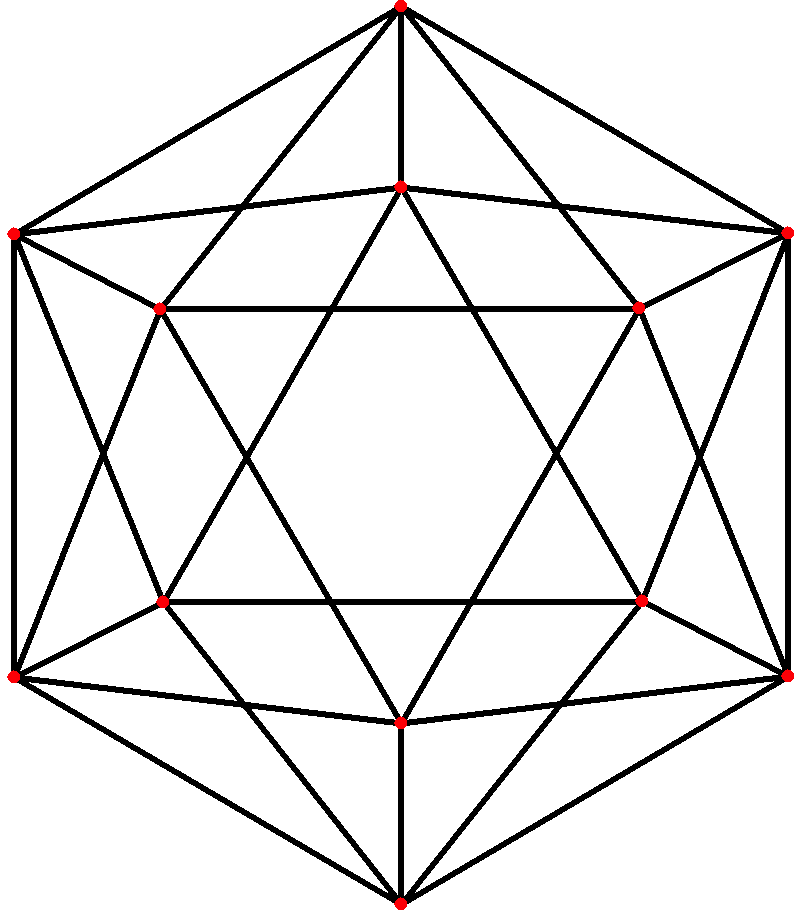
\includegraphics{hypercomp/Icosahedron.png}
  \caption{An icosahedron.}
  \label{fig:icosahedron}
\end{marginfigure}
A similar approach can be used to make an ambisonic level
detector. However, a compressor needs to react much quicker than a
level meter. The compressor cannot even \emph{begin} to engage until
the level meter has responded, and attack times faster than 33
milliseconds are common in conventional compression. Every point on
the sphere requires a buffer to calculate the RMS. We also need to
decode ambisonics at the audio sample rate and keep track of peak
values. Ideally we would also interpolate between the points.

\subsection{An Efficient Level Detection Module}
\label{sec:hyperc-level-detect}
The Hypercompressor needs to detect the level of our ambisonic input
material and identify (as quickly as possible) when and where the
signal exceeds the compressor threshold. In the interest of
computational efficiency, the first level detector I wrote attempted
to extract overage information with minimal ambisonic decoding and
signal processing.
\begin{enumerate}
\item To accurately play a first order ambisonic encoding, we need a
  minimum of 6 speakers placed around the listener. In this level
  detector, we calculate the root mean square (RMS) average at the
  center of 6 lobes corresponding to the first order spherical
  harmonics: front, rear, left, right, top, and bottom.
\item Calculate a map of the influence of each lobe on the surround
  image\TODO{Clean}
  (figures~\ref{fig:hypercomp-mathematica},~\ref{fig:hypercomp-inf-maps}). For
  example, pan a monophonic sound directly forward in an ambisonic
  mix, cache an image of the resulting sound sphere. Save one image
  for each of the 6 lobes.
\item We have 6 images, each representing one of the 6 lobes of our
  first order ambisonic spherical harmonics. In step 1, we calculated
  the RMS level at each of the corresponding points on our surround
  sphere. Use the 6 RMS levels to weight each of our 6 maps. The sum
  of the weighted maps shows the gain distributed across our ambisonic
  sphere.
\end{enumerate}

\begin{figure}[]
  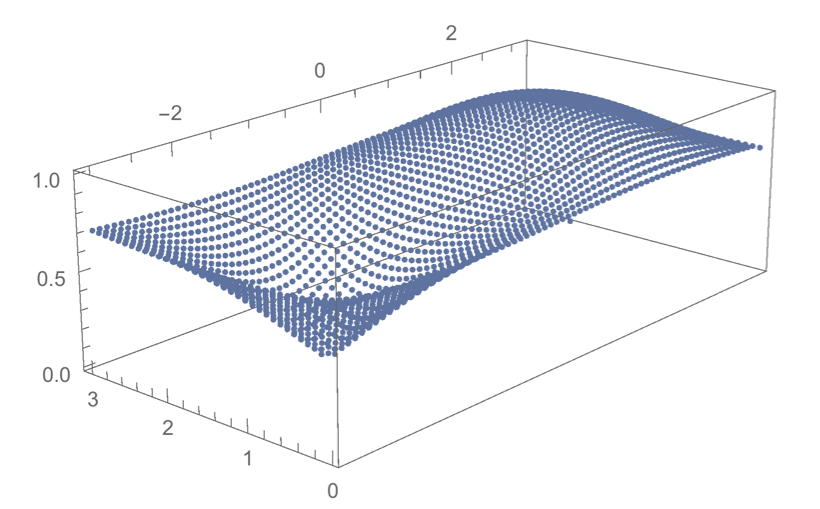
\includegraphics[width=\linewidth]{hypercomp/AmbisonicFieldAngle.png}
  \caption{Calculating the cylindrical projection of single ambisonic panned
    source in the Wolfram Mathematica software package}
  \label{fig:hypercomp-mathematica}
\end{figure}

\begin{figure}[]
 
\includegraphics[width=3.5cm]{hypercomp/left_x72.png}
 
\includegraphics[width=3.5cm]{hypercomp/above_x72.png}
 
\includegraphics[width=3.5cm]{hypercomp/front_x72.png}
 % 
\includegraphics[width=3.5cm]{hypercomp/right_x72.png}
 % 
\includegraphics[width=3.5cm]{hypercomp/below_x72.png}
 % 
\includegraphics[width=3.5cm]{hypercomp/rear_x72.png}
  \caption{Influence maps of 3 first-order spherical harmonics: left, top, and
    front. Pure white is $-0$~dBFS black is -inf~dBFS. Cylindrical projection.}
  \label{fig:hypercomp-inf-maps}
\end{figure}

\paragraph{Ambisonic Efficient Level Detection Module Results}If the
input to the level detector is encoded as an ambisonic plane wave,
this level detector does yield accurate results.  In the more common
case, when our ambisonic input material contains multiple sources that
are each ambisonically panned to different positions, this
interpolation technique does not accurately calculate the RMS at any
angle. In simple cases, where we can be sure our input material is
appropriate, the technique described here might be useful, but in most
cases, a different approach will be more effective.

\begin{figure}[h]
%  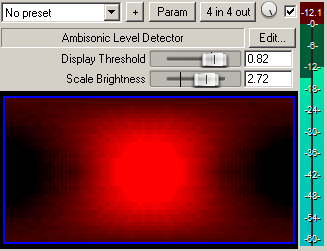
\includegraphics{hypercomp/LevelDetect_front.png}
  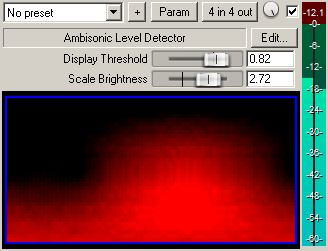
\includegraphics{hypercomp/LevelDetect_45_down.png}
  \caption{The Hypercompressor visualizer written for the efficient
    ambisonic level detector. The surround sphere is projected to a
    cylinder and unwrapped on the flat surface. In this image, a
    monophonic source is panned slightly down and to the right
    ($45\degree$~azimuth, $-45\degree$~elevation).}
  \label{fig:hypercomp-inf-map-angle}
\end{figure}

\subsection{Ambisonic Gain Control Module}
\label{sec:ambis-gain-contr}
The spherical harmonics defined in equation~\ref{eq:ambisonics} form a
set of orthogonal basis functions. If we define a sequence for our
spherical harmonics and spherical harmonic expansion coefficients, we
can treat a set of expansion coefficients as a vector, and perform
matrix operations on them that rotate, warp, and re-orient our
three-dimensional surround sound image.\cite{Pomberger2011} The
ability to mathematically warp and manipulate our surround sound image
makes ambisonics the perfect choice for implementing a surround sound
compressor.

\paragraph{The Focus Transform} One transform that lets us attenuate a
region of the surround sound sphere is the \textit{focus} transform
distributed as part of the open source Ambisonic Toolkit
(ATK).\sidenote{\url{http://www.ambisonictoolkit.net/}}\cite{Anderson2009}
\begin{equation}
F(w)=\left( \begin{array}{cccc}
\frac{1}{1 + \sin|w|} & 
\frac{1}{\sqrt{2}} \frac{\sin(w)}{1 + \sin|w|}  & 
0 &
0 \\
\sqrt{2}\frac{sin(w)}{1 + \sin|w|} & % LG1
\frac{1}{1 + \sin|w|} &                    % LG0
0 & 
0 \\
0 & 
0 &
\frac{\cos(w)}{1 + \sin|w|} &
0 \\
0 &
0 &
0 &
\frac{\cos(w)}{1 + \sin|w|} 
\end{array} \right)
\label{eq:focus}
\end{equation}
This transform is intended to focus attention on the region directly
in front of the listener ($0\degree$ azimuth, $0\degree$ elevation),
by attenuating the region in the opposite direction, and gently
warping the surround image toward the front. $w$ is a value between
$0$ and $\frac{\pi}{2}$~radians, and specifies the intensity of the
transformation. When $w=0$, the surround field is unchanged. When
$w=\frac{\pi}{2}$ sounds panned hard to the rear are muted, sounds
panned to the left and right will be attenuated by 6dB, the entire
surround image is warped to the front, and the gain facing forward is
unchanged. This enables us to push one sound out of the way to make
room for another sound as described in
section~\ref{sec:hypercomp-design}.

Equation~\ref{eq:focus} attenuates the region behind the listener. 
If we want to attenuate a region other than the rear, we can rotate
$F$ using a rotation matrix like the one below.
\begin{equation}
R_z(\varphi)=\left( \begin{array}{cccc}
1 & 0 & 0 & 0 \\
0 & \cos(\varphi) & \sin(\varphi) & 0 \\
0 & -sin(\varphi) & cos(\varphi) & 0 \\
0 & 0 & 0 & 0
\end{array} \right)
\label{eq:rotation}
\end{equation}
Equation~\ref{eq:rotation} (from the ATK) describes a rotation around
the z-axis, by $\varphi$ radians. To rotate the focus transform to the
right instead of to the front, we first apply the focus transform to
the inverse of a $90\degree$ right rotation. Then we apply the
$90\degree$ matrix to the result. This example is generalized by:
\begin{equation}
X(w,\varphi,\vartheta)=R_z(\varphi)R_y(\vartheta)F(w) R_y^{-1}(\vartheta)R_z^{-1}(\varphi)
\label{eq:comp-focus}
\end{equation}
Equation~\ref{eq:comp-focus} lets us programmatically generate an
ambisonic focus transform matrix that targets a specified region of
the surround field, fulfilling the objectives for our ambisonic gain
control module in the Hypercompressor.

\paragraph{Ambisonic Gain Control Module Results}
The focus transform lets us warp the surround field, pushing the
field to make room for new sounds. In some cases (for example, when
mastering an ambisonic recording) warping the surround image is
undesirable, and a simple directional gain transform should be used
instead (an appropriate transform is defined
elsewhere\cite{Kronlachner2014i}). However, the goal of the
Hypercompressor is not to compress dynamic range like a traditional
compressor. The goal is to compress \emph{space}. The focus transform
is a compromise: We partly attenuate a region, but we also bend the
surround image so that important parts of our surround texture are
panned to a position with fewer competing sounds. This is an effect
that is not possible with a traditional compressor.

The focus transform also ties attenuation amount to attenuation
radius. If we use only a single focus transform, is not possible to only
slightly attenuate a large region of the surround sound field. The
following chapter describes how we used this to our advantage
during the live performance of \textit{De L'Exp\'{e}rience}.

%%% Local Variables:
%%% mode: latex
%%% TeX-master: "CharlesHolbrow_MAS_Thesis"
%%% End:
